%!TEX root = ../crimson_throne_book_main.tex
% 2015-08-01
And so the companions return to Endrin military academy, with Amin Jalento in tow. Again, the only thing answering their call at the front doors is a dog barking inside. Quint uses the Key-lock Killer's bell to magically open the entrance. The barking comes from a room down the hall.\hyperref[fig:Endrin-military-academy-550435227]{ It leads the young friends to a training room } where a white labrador retriever sinks into a low growl. Balian sends Spyder over to ease the animal's discomfort, as suddenly one of the practice dummies comes to life and jumps down from \hyperref[fig:Ambush-in-the-training-room-550436061]{ the wooden scaffolding and swings his longsword at Quint } . "Get out, intruders. We don't need looters in here!" He draws some blood, but when the bard looks at the man's face, he notices a long scar across his left cheek. When Danarella talked about Janros Rainwater, she mentioned such a distinct scar. \\

\begin{figure}[h]
	\centering
	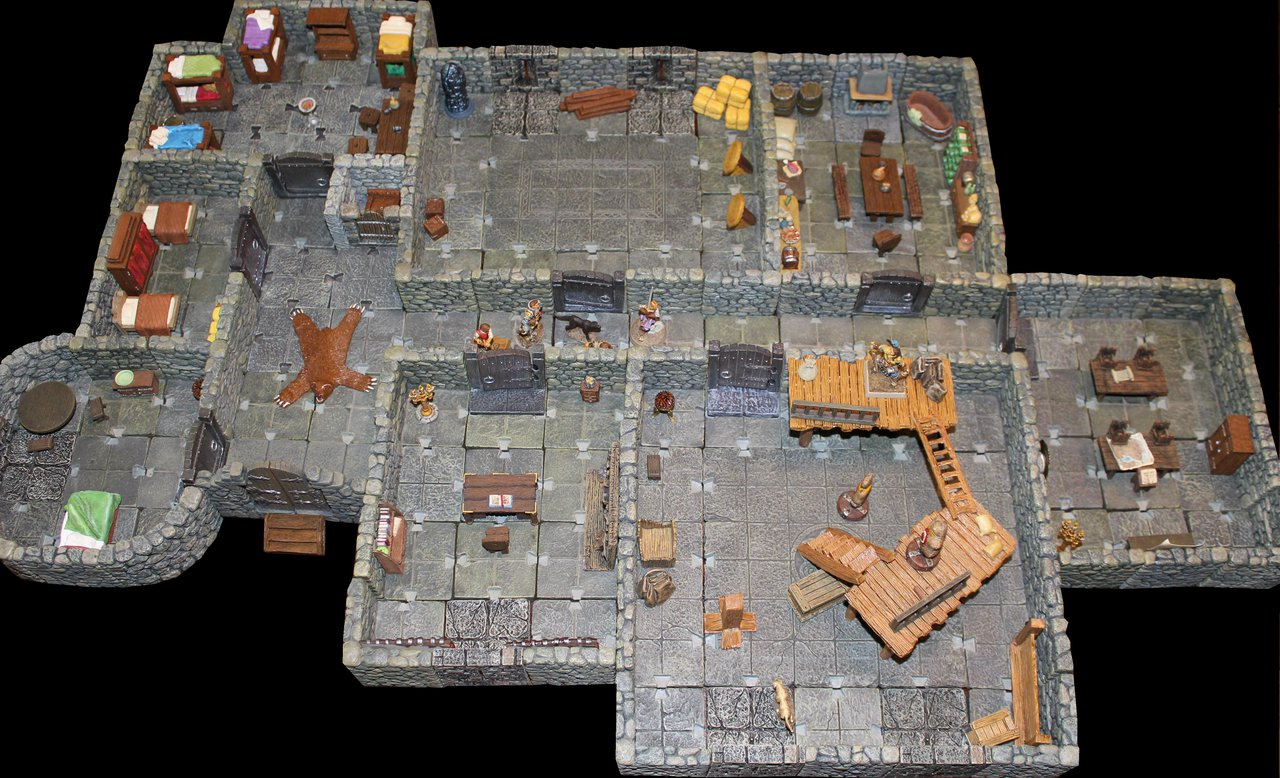
\includegraphics[width=0.39\textwidth]{images/Endrin-military-academy-550435227.jpg}
	\caption{Endrin military academy}
	\label{fig:Endrin-military-academy-550435227}
\end{figure}

\begin{figure}[h]
	\centering
	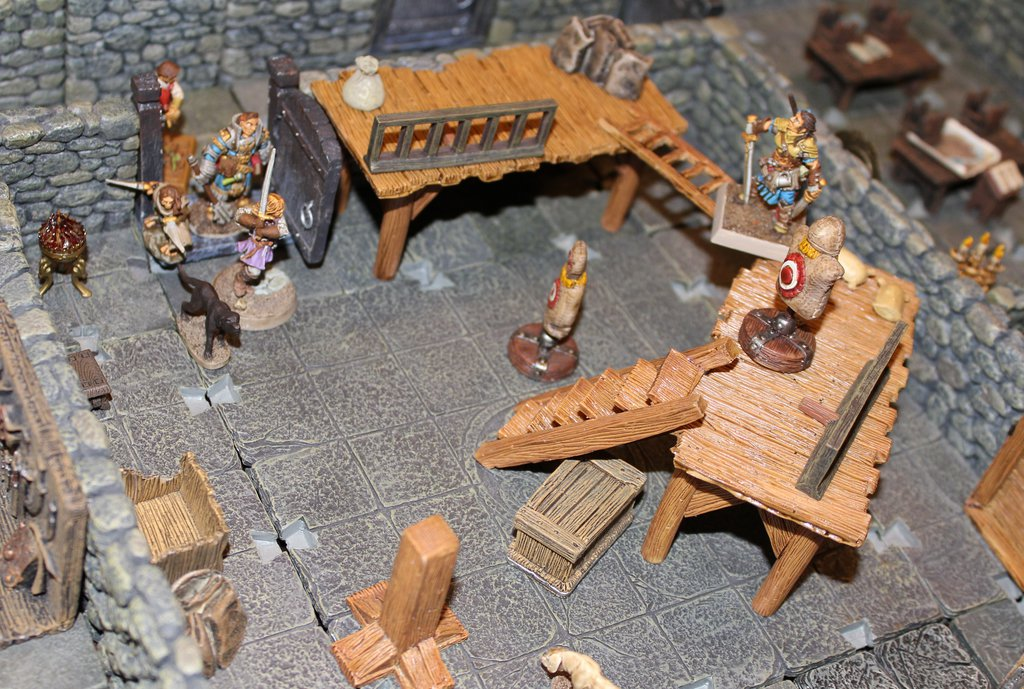
\includegraphics[width=0.39\textwidth]{images/Ambush-in-the-training-room-550436061.jpg}
	\caption{Ambush in the training room}
	\label{fig:Ambush-in-the-training-room-550436061}
\end{figure}

"We come in peace ... Janros Rainwater, I presume. We're not here to steal from you, we're here to talk. We want to ask you about Yuuna", the bard says.\\

"Yuuna, do you know where she is?" he jumps to Quint's words.\\

"We were actually hoping you might tell us", Quint continues with a slight tone of disappointment.\\

"She's been missing for a couple of days now, she hasn't been at work and she's not at home."\\

"So you've been to her place. Maybe you're the one who got in through the back window", Sjo speculates.\\

"Indeed I was. The only thing I found was a wooden toy house, representing a local little restaurant. I don't know if you're familiar with it, 'The Traveling Man' it's called. I went there and asked about her, but I didn't find anything."\\

"So, you're here all by yourself, or what?" Balian notices.\\

"Just me and Boomer", Janros pets the dog. "Everyone else was called back into service, when all the trouble started after King Eodred died. I am one of the seniors here, so I stayed behind to keep an eye on things. There have been a couple of attempts at looting since the quarantine. That is why I attacked you ... I do apologize, of course."\\

"Don't worry about it, hard times demand even harder measures. We understand," Quint assures the man." Still, I imagine you do not know what is happening to your brethren on the mainland. They are much worse off."\\

"My brothers, what do you mean?"\\

"Well, there is no easy way to break this news to you," Sjo explains. "The Sable Company has been outlawed after Commander Endrin attempted to murder the queen."\\

"He did what?"\\

"He tried to kill her, shot an arrow straight into her head, he did", Balian goes on. "Should have killed her on the spot, but she pulled it out like it was a splinter and planted it right between Endrin's eyes. Game over for him, and his troops with him. The Gray Maidens have been all over town hunting the Sable Company down."\\

"By the gods, I must get over there and help them!" Janros shouts.\\

"If some of your colleagues are still alive and at large, they've probably gone into hiding already. There's not much you can do", Quint says.\\

"The hell there isn't. I cannot sit idle while my friends are being butchered or arrested. I have to help, or at least I have to try!" Janros objects.\\

"Why don't you come with us to find Yuuna?" Sjo suggests.\\

"As much as I love her, duty calls. I'll give you the wooden house, though I don't see what good it will do. Then I have to go."\\

The toy house does not only portray 'The Travelling Man', but also the square in front of it, which is famous for its occasional otyugh outbursts. A small wooden circle represents the plug over the sewer entrance. Puk notices he can remove it and sees a strange, vaguely heart shaped indentation underneath it. Studying it, Quint realizes that it perfectly fits the feet of the wooden Yuuna figurine. So she is not in 'The Travelling Man' after all, but in the nearby sewers!\\

The companions quickly say goodbye to Janros Rainwater and Amin Jalento, who has agreed to watch over the Endrin academy in Janros's absence. Afterwards they hurry to the square in front of 'The Travelling Man'. A heavy grid covers a substantial hole in the ground, which is normally winched open every Oathday to feed the garbage eaters. Next to this giant plug is a smaller manhole with a lid, which opens easily, revealing a ladder down. A scared female voice rings from below: "Is anyone there? Please help me!" The slightly exotic accent betrays her Vudran heritage. It is Yuuna! And she is still alive!\\

The adventurers climb down and\hyperref[fig:Otyugh-sewer-pit-Korvosa-550449437]{ find a stone set of stairs leading further into the dark } . Below a light shines from a locked cage which houses a scared woman. She clings to the bars in the front, trying to avoid the tentacles swinging at her in the back of the cage. A hungry otyugh is barred from entering at the other end, but it is attempting to grab the Vudran with its long feelers through the iron ribs. \\

\begin{figure}[h]
	\centering
	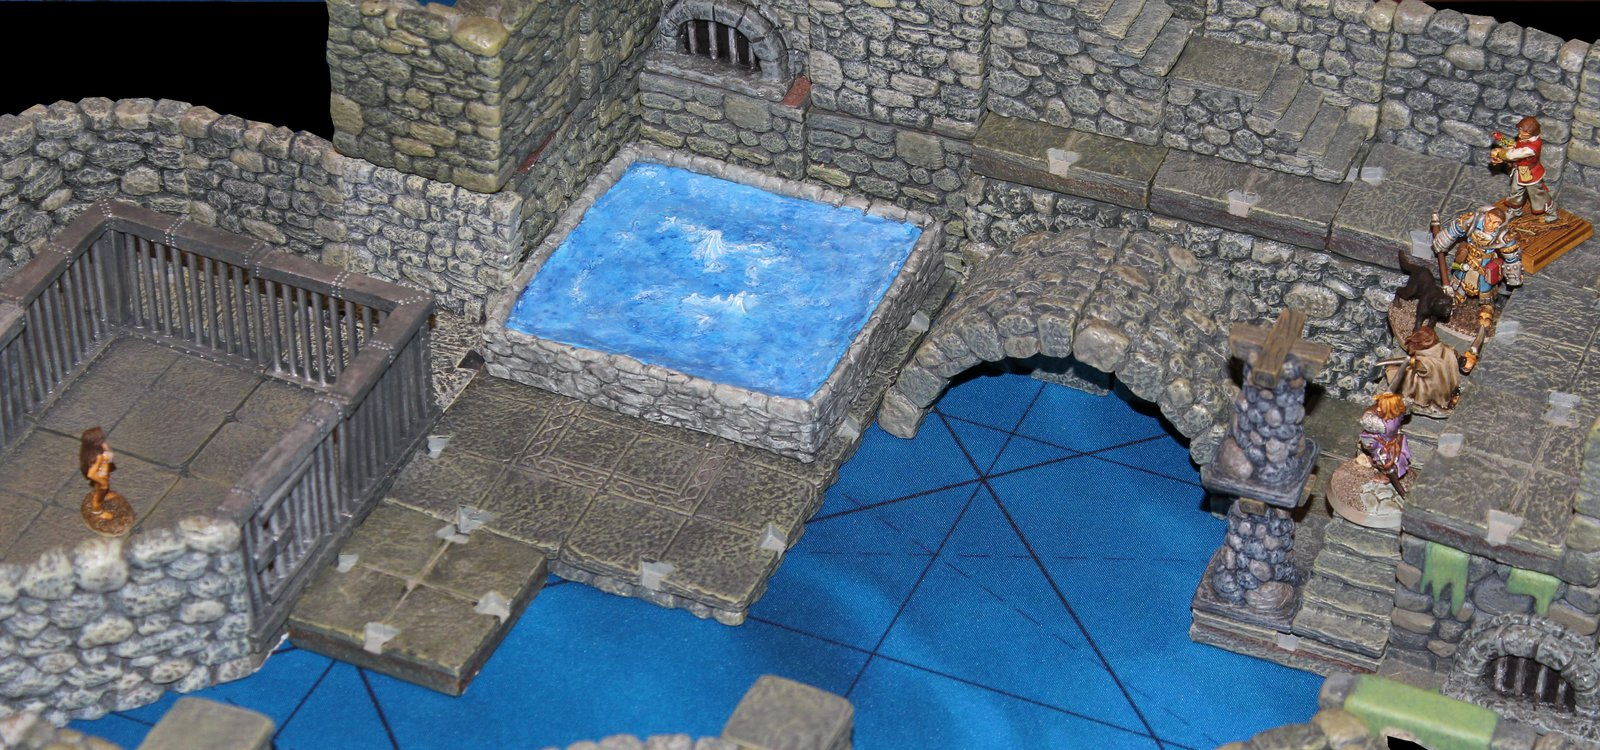
\includegraphics[width=0.39\textwidth]{images/Otyugh-sewer-pit-Korvosa-550449437.jpg}
	\caption{Otyugh sewer pit Korvosa}
	\label{fig:Otyugh-sewer-pit-Korvosa-550449437}
\end{figure}

Then a second female voice calls out: "Once again we bear witness to your slow and feeble attempts at rescuing those you love! You should have been here hours ago! Still, I'll give you this one shot at saving the damsel in distress to kick off our little game. There will be no such mercy from here on, though. So, prove to me how fast you are at rescuing your friends or watch them die! No time to dally." With the sound of metal grinding on stone several portcullises rise and at the same time the door in the back of Yuuna's cage swings open, clearing the way for the otyugh to charge in.\\

"Puk, use the {\itshape cloak of the pixie king} !" Quint shouts as everyone gathers around the halfling who zaps the party into the cage. Arriving behind the bars gives the companions the opportunity to confront Yuuna's foe, but it also keeps them safe from the pair of otyughs that enter the central room through the other opened passages, or at least the heroes think so, because the creatures simply stretch their appendices through the iron poles to attack. Balian cuts a deep slash into the sewer monster in the cage, but then he sees an extraordinarily large specimen emerging from one of the lower pipes. \hyperref[fig:Otyugh-attack-in-Old-Korvosa-550450012]{ The creature glides its mighty tentacle through the bars and grabs the ranger with it } , pulling him against the iron and crushing his ribs. Quint tries to save his friend by nauseating the huge grappler with  {\itshape cacophonous call} , but his magic is easily resisted. One of the normal sized beasts also grabs Balian through the metal, putting the ranger in dire straits. Inside the cage the otyugh bites Sjo with its filthy teeth, but it doesn't survive Puk's deadly gashes. Next Sjo draws upon his mastery over the element of fire and hurls a  {\itshape fireball} at the three monsters in the central room. Burned sewage is not exactly a pleasant smell, but the crisp meat on the otyughs' backs is definitely a welcome sight. Balian fails to free himself from the huge tentacle and has to resort to his dagger to gash the tendril that squeezes him. It takes several rounds of cutting and two extra  {\itshape fireballs} to drop another otyugh and send the two remaining ones running. \\

\begin{figure}[h]
	\centering
	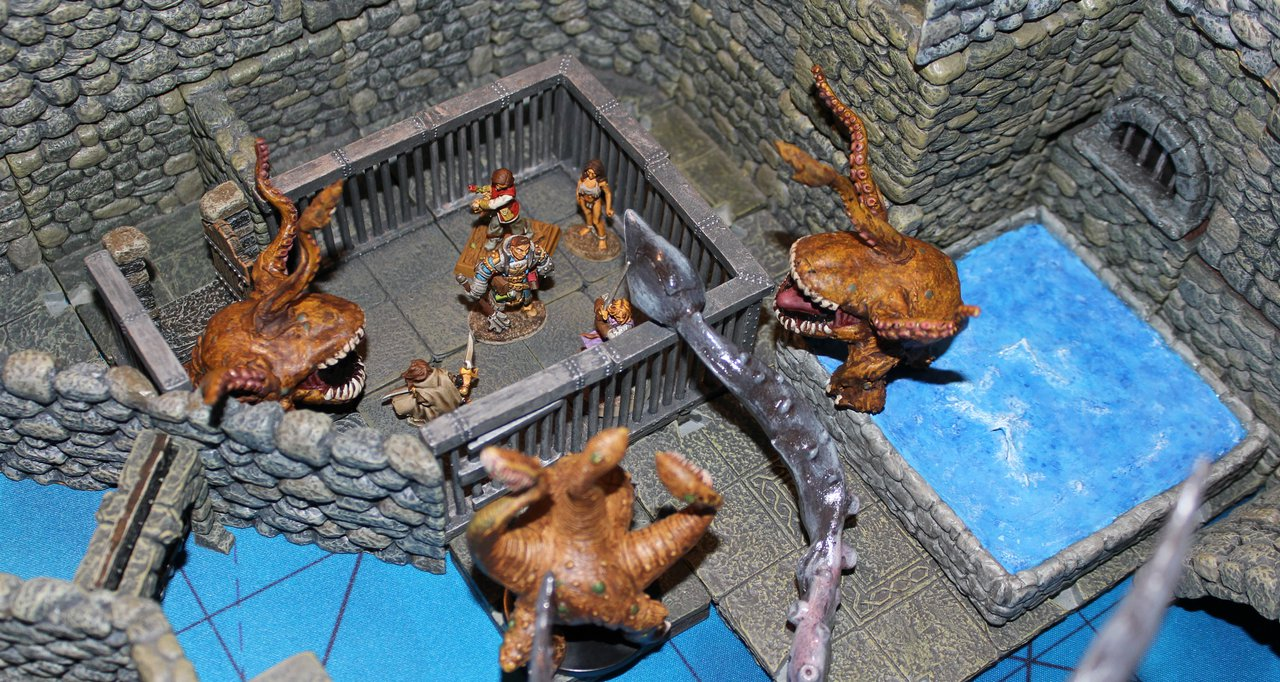
\includegraphics[width=0.39\textwidth]{images/Otyugh-attack-in-Old-Korvosa-550450012.jpg}
	\caption{Otyugh attack in Old Korvosa}
	\label{fig:Otyugh-attack-in-Old-Korvosa-550450012}
\end{figure}

While Yuuna thanks Quint profusely for saving her, Balian notices another toy house in the corner. This one resembles the temple of Aroden, an old crumbling church, devoted to the worship of the city's former most popular god, until he disappeared a century ago. A pitiful trio of clerics is rumored to maintain the building as best they can, going so far as to hold services every Sunday for a handful of patrons, most of whom are not worshippers, but simply curious observers. The feet of the Korwick doll fit into an indentation inside the wooden miniature building.\\

